\chapter{ANALISIS DAN PERANCANGAN SISTEM}
\vspace{1em}

\section{Deskripsi Sistem}
Sistem yang dikembangkan dalam penelitian ini merupakan sebuah aplikasi pemodelan gerak tari tradisional Indonesia dengan memanfaatkan teknologi \textit{pose estimation} dan robot \textit{humanoid} ROBOTIS-OP3. Sistem ini dirancang untuk mengekstraksi gerakan manusia dari video tari tradisional, menerjemahkannya ke dalam data koordinat 3D tubuh manusia, kemudian mengonversinya menjadi pergerakan fisik pada robot \textit{humanoid}.

Proses utama dari sistem dimulai dari input berupa video tari tradisional Indonesia yang dianalisis menggunakan model \textit{pose estimation} berbasis \textit{deep learning}. Model awal menggunakan pendekatan Metrabs (METa-learning TRAnsformer for 3D human pose eStimation) untuk menghasilkan koordinat pose 3D dari setiap frame dalam video, kemudian disempurnakan dengan metode DeciWatch yang meningkatkan akurasi dan kelancaran gerakan melalui pendekatan \textit{sample-denoise-recover}. Hasil estimasi berupa data \textit{keypoints} 3D kemudian dikonversi menjadi sudut-sudut servo (\textit{servo angles}) menggunakan algoritma \textit{Inverse Kinematics} (IK), dan seluruh data gerak tersebut disimpan dalam format file seperti JSON. File ini dapat digunakan untuk input kontrol robot \textit{humanoid} ROBOTIS-OP3 secara terpisah melalui sistem eksekusi gerak yang terintegrasi dengan ROS, sehingga memungkinkan robot untuk mereplikasi gerakan tari secara bertahap sesuai instruksi dalam file tersebut.

\section{Analisa Kebutuhan Sistem}

Dalam membangun sistem pemodelan gerak tari tradisional berbasis \textit{pose estimation}, dilakukan analisa kebutuhan terhadap perangkat keras (\textit{hardware}) dan perangkat lunak (\textit{software}) yang digunakan dalam proses pengolahan data, pelatihan model, serta integrasi dengan robot \textit{humanoid} ROBOTIS-OP3. Kebutuhan ini ditentukan berdasarkan tingkat kompleksitas komputasi dan kompatibilitas sistem.

\subsection{Kebutuhan Perangkat Keras}
Perangkat keras yang digunakan dalam penelitian ini terdiri dari laptop/PC untuk pengolahan data dan robot \textit{humanoid} ROBOTIS-OP3 sebagai platform eksekusi gerakan. Spesifikasi perangkat keras yang dibutuhkan adalah sebagai berikut:

\begin{longtable}{|c|p{9cm}|}
    \caption{Spesifikasi Perangkat Keras Laptop}
    \label{tab:spesifikasi_laptop} \\
    \hline
    \textbf{No} & \textbf{Nama Perangkat Keras} \\
    \hline
    \endfirsthead
    
    % \hline
    % \textbf{No} & \textbf{Nama Perangkat Keras} \\
    % \hline
    \endhead
    
    \hline
    \endfoot
    
    \hline
    \endlastfoot
    
    1 & Intel Core i5 Gen-10 \\ \hline
    2 & NVIDIA GeForce RTX 3060 6GB Mobile \\ \hline
    3 & RAM 16GB \\ \hline
    4 & SSD 256GB \\ \hline
    
\end{longtable}
    
\begin{longtable}{|c|p{9cm}|}
    \caption{Spesifikasi Perangkat Keras Robot}
    \label{tab:spesifikasi_robot} \\
    \hline
    \textbf{No} & \textbf{Nama Perangkat Keras} \\
    \hline
    \endfirsthead
    
    % \hline
    % \textbf{No} & \textbf{Nama Perangkat Keras} \\
    % \hline
    \endhead
    
    \hline
    \endfoot
    
    \hline
    \endlastfoot
    
    1 & Intel Core i3-7100U \\ \hline
    2 & RAM 8GB \\ \hline
    3 & SSD 256GB \\ \hline
    4 & Dynamixel XM430-W350, 2XL430-W250 \\ \hline
    
\end{longtable}
        
\subsection{Kebutuhan Perangkat Lunak}
Perangkat lunak yang digunakan dalam penelitian ini meliputi sistem operasi, bahasa pemrograman, dan berbagai pustaka (\textit{library}) yang mendukung pengolahan data, pelatihan model, serta komunikasi dengan robot. Berikut adalah spesifikasi perangkat lunak yang dibutuhkan:

\begin{longtable}{|c|p{5cm}|p{8cm}|}
    \caption{Spesifikasi Perangkat Lunak}
    \label{tab:kebutuhan_perangkat_lunak} \\
    \hline
    \textbf{No} & \textbf{Nama} & \textbf{Keterangan} \\
    \hline
    \endfirsthead
    
    % \hline
    % \textbf{No} & \textbf{Nama} & \textbf{Keterangan} \\
    % \hline
    \endhead
    
    \hline
    \endfoot
    
    \hline
    \endlastfoot
    
    1 & Sistem Operasi Laptop & Ubuntu 24.04 LTS \\ \hline
    2 & Sistem Operasi Robot & Linux Mint 16 \\ \hline
    3 & Bahasa Pemrograman & Python 3.9, C++, Bash \\ \hline
    4 & Text Editor & Visual Studio Code, Nano \\ \hline
    5 & Pustaka Pemrograman & TensorFlow, PyTorch, NumPy, OpenCV, Matplotlib, Flask \\ \hline
    6 & Robot Operating System & ROS Kinetic, ROS 2 Humble \\ \hline
    7 & Perangkat Lunak Pendukung & Jupyter Notebook, Google Colab \\ \hline
    
\end{longtable}
    

\subsection{Analisa Kebutuhan Fungsionalitas}

Analisis kebutuhan fungsional merupakan proses identifikasi dan dokumentasi terhadap fitur dan fungsi spesifik yang harus dimiliki oleh sistem. Proses ini bertujuan untuk mendefinisikan tugas-tugas utama yang dilakukan oleh sistem, cara sistem berinteraksi dengan pengguna, serta bagaimana sistem merespons input yang diterima. Kebutuhan ini menjadi dasar dalam proses perancangan dan implementasi sistem secara keseluruhan, sebagaimana ditunjukkan pada Tabel~\ref{tab:kebutuhan_fungsionalitas}.

\begin{longtable}{|c|p{5cm}|p{8cm}|}
\caption{Kebutuhan Fungsional Sistem}
\label{tab:kebutuhan_fungsionalitas} \\
\hline
\textbf{No} & \textbf{Fungsi} & \textbf{Deskripsi} \\
\hline
\endfirsthead

\hline
\textbf{No} & \textbf{Fungsi} & \textbf{Deskripsi} \\
\hline
\endhead

\hline
\endfoot

\hline
\endlastfoot

1 & Upload Video & Sistem menyediakan fitur bagi pengguna untuk mengunggah video tari tradisional Indonesia dalam format umum seperti MP4 atau AVI. Nama file akan tampil pada area log sebagai konfirmasi. \\
\hline
2 & Estimasi Pose dan Filtering & Sistem melakukan proses estimasi pose tubuh manusia dalam bentuk koordinat 3D \textit{keypoints} menggunakan model MeTRAbs dan DeciWatch. Hasil estimasi difilter untuk mengurangi noise pada prediksi temporal. \\
\hline
3 & Visualisasi Skeleton 3D & Sistem menampilkan hasil estimasi pose dalam bentuk skeleton 3D yang divisualisasikan sesuai urutan frame video. \\
\hline
4 & Status Log & Sistem mencatat dan menampilkan status proses seperti upload, estimasi, dan penyimpanan pada area log agar pengguna dapat memantau jalannya sistem. \\
\hline
5 & Penyimpanan Data & Sistem menyimpan hasil estimasi pose ke dalam file berformat JSON yang dapat digunakan untuk kontrol robot. File ini akan disimpan di direktori output. \\
\hline
6 & Playback Robot & Sistem mengontrol robot ROBOTIS-OP3 untuk mereproduksi gerakan berdasarkan file JSON hasil estimasi. Robot akan bergerak sesuai urutan sudut artikulasi yang dihasilkan dari \textit{motion retargeting}. \\
\hline

\end{longtable}


\section{Perancangan Sistem}

Perancangan sistem dilakukan untuk mendefinisikan bagaimana komponen-komponen dalam sistem saling berinteraksi dan berfungsi dalam keseluruhan proses pemodelan gerak tari tradisional menggunakan teknologi \textit{pose estimation}. Sistem ini dirancang dengan pendekatan modular, mulai dari tahap akuisisi video hingga penyimpanan data gerakan dalam format yang dapat dieksekusi oleh robot \textit{humanoid} ROBOTIS-OP3.

\subsection{Arsitektur Sistem}

\begin{figure}[H]
    \centering
    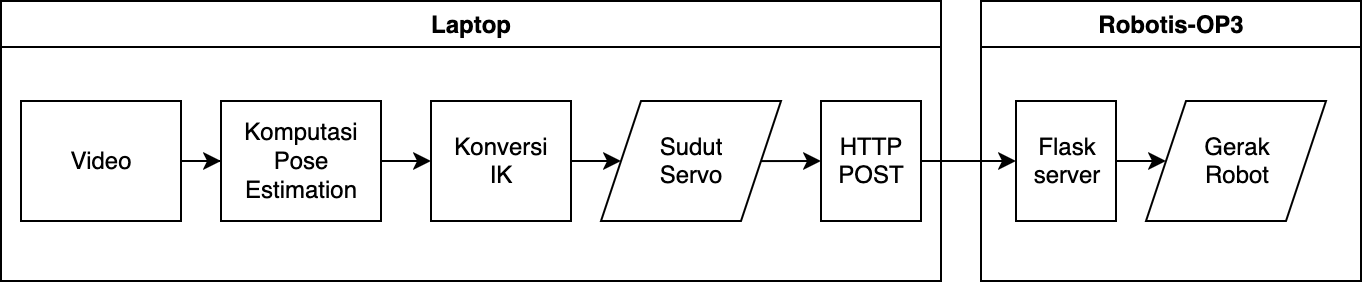
\includegraphics[width=0.9\textwidth]{images/arsitektur_sistem.png}
    \caption{Diagram Arsitektur Sistem}
    \label{fig:arsitektur_sistem}
\end{figure}

Gambar~\ref{fig:arsitektur_sistem} menunjukkan arsitektur sistem yang dikembangkan untuk pemodelan gerak tari tradisional menggunakan teknologi \textit{pose estimation}. Sistem ini terdiri dari dua bagian utama, yaitu pemrosesan data pada laptop dan eksekusi gerakan pada ROBOTIS-OP3.

Pada sisi laptop, input berupa video tari diproses melalui modul komputasi estimasi pose untuk memperoleh koordinat 3D tubuh manusia. Data koordinat ini kemudian dikonversi menggunakan algoritma \textit{Inverse Kinematics} (IK) menjadi sudut servo yang sesuai dengan struktur pergerakan robot. Sudut servo tersebut dikemas dalam format \textit{JSON} dan dikirimkan ke robot melalui protokol komunikasi \textit{HTTP POST} menggunakan \textit{Flask client} di sisi laptop.

Sementara itu, di sisi robot ROBOTIS-OP3, data gerakan diterima oleh \textit{Flask server}, kemudian disimpan dalam format file JSON sebagai rekaman gerak. Data ini digunakan untuk mengontrol aktuator robot sehingga menghasilkan gerakan yang sesuai dengan video input. Pendekatan ini memanfaatkan pemisahan beban komputasi, di mana proses komputasi berat dilakukan di laptop, sedangkan robot fokus pada eksekusi pergerakan. Metode ini juga memudahkan integrasi sistem dan pengujian karena menggunakan protokol \textit{HTTP} yang lebih sederhana dan fleksibel dibandingkan komunikasi \textit{socket}.



\subsection{Alur Kerja Sistem}

\begin{figure}[H]
    \centering
    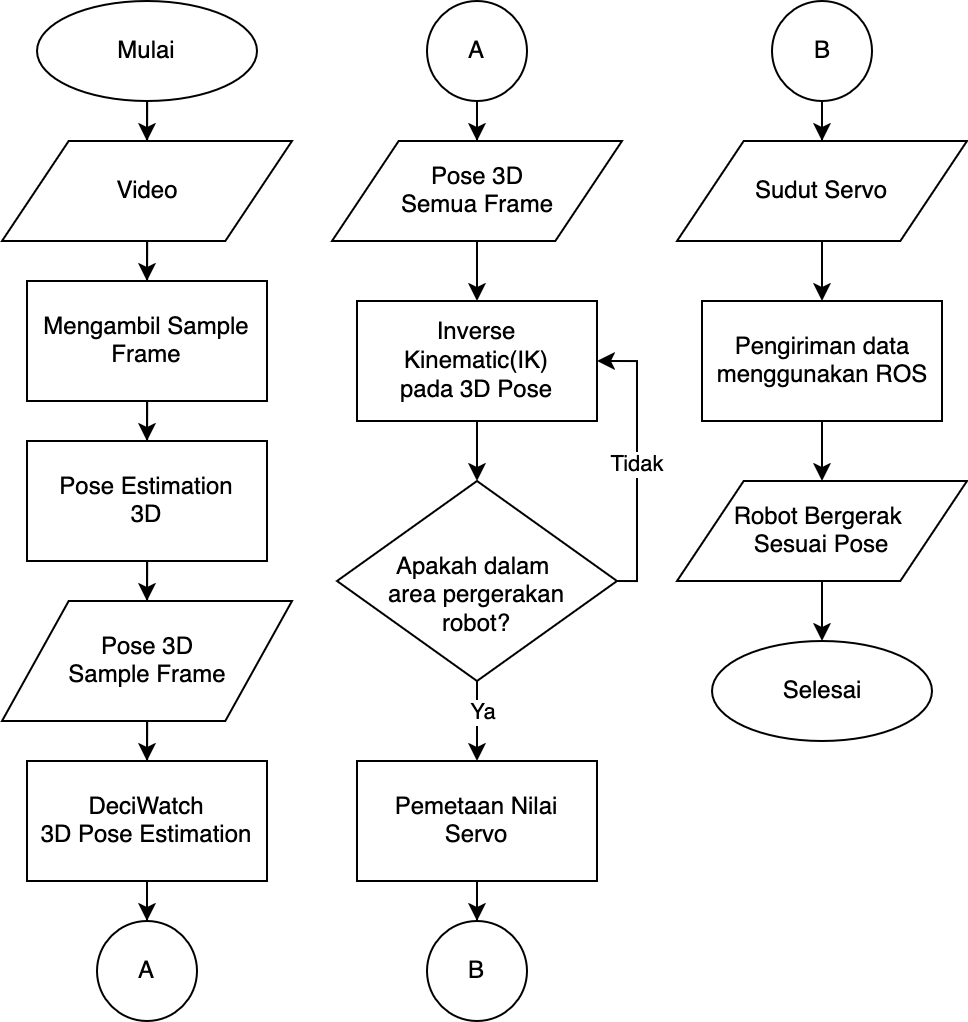
\includegraphics[width=0.8\textwidth]{images/system_flowchart.png}
    \caption{Flowchart Perancangan Sistem}
    \label{fig:flowchart_sistem}
\end{figure}

Gambar \ref{fig:flowchart_sistem} menunjukkan alur kerja sistem yang dirancang dalam penelitian ini, dimulai dari input video hingga eksekusi gerakan oleh robot \textit{humanoid} ROBOTIS-OP3. Berikut adalah penjelasan rinci tiap langkah dalam alur sistem:

\begin{enumerate}
    \item {Input Video} \\
    Sistem menerima masukan berupa video tari tradisional Indonesia dalam format umum seperti MP4.
    
    \item {Pengambilan Sampel Frame} \\
    Video diolah dengan mengambil sampel beberapa frame secara berkala untuk mengurangi beban komputasi dan menyesuaikan dengan kebutuhan input model.
    
    \item {Pose Estimation 3D} \\
    Setiap frame hasil sampel diproses menggunakan model \textit{pose estimation} berbasis Metrabs untuk menghasilkan prediksi koordinat 3D dari titik-titik persendian tubuh manusia. Sistem mendukung dua jenis model \textit{skeleton}, yaitu \textit{LSP-14} yang terdiri dari 14 titik persendian utama dan \textit{COCO-19} yang terdiri dari 19 titik, sehingga dapat disesuaikan dengan kebutuhan pemetaan gerakan pada robot.
    
    \item {DeciWatch 3D Pose Estimation} \\
    Output pose 3D dari Metrabs kemudian diolah lebih lanjut menggunakan DeciWatch. Model ini melakukan prediksi berurutan (temporal) untuk memastikan kontinuitas dan kelancaran gerakan antar-frame, sehingga menghasilkan estimasi pose 3D yang lebih halus.
    
    \item {Inverse Kinematics (IK) pada 3D Pose} \\
    Seluruh pose 3D hasil prediksi kemudian dikonversi menjadi sudut sendi menggunakan metode \textit{Inverse Kinematics Transform (IKT)}. Perhitungan ini dilakukan untuk mendapatkan sudut aktuator yang diperlukan agar robot dapat menirukan pose tersebut.
    
    \item {Validasi Area Pergerakan Robot} \\
    Sistem memeriksa apakah hasil perhitungan IK berada dalam jangkauan aktuator robot untuk menghindari servo bertabrakan. Jika tidak, maka pose akan disesuaikan agar tetap dalam batas gerak yang dapat dieksekusi oleh ROBOTIS-OP3 dengan cara membatasi sudut tersebut.
    
    \item {Pemetaan Nilai Servo} \\
    Setelah validasi, hasil IK dipetakan menjadi nilai sudut servo sesuai dengan konfigurasi servo pada robot.
    
    \item {Pengiriman Data ke Robot} \\
    Nilai sudut servo yang telah dihasilkan dari proses \textit{motion retargeting} dikirimkan ke robot menggunakan metode komunikasi berbasis HTTP POST. Data sudut servo dikemas dalam format \textit{JSON} dan dikirimkan melalui jaringan ke alamat IP robot.
    
    \item {Eksekusi Gerakan Robot} \\
    Robot ROBOTIS-OP3 akan mereplikasi gerakan sesuai dengan urutan pose yang telah dikirimkan, sehingga mampu merepresentasikan gerakan tari dalam bentuk fisik secara otomatis.
\end{enumerate}

Dengan alur ini, sistem secara menyeluruh dapat mengonversi gerakan manusia dari video menjadi pergerakan robot yang menyerupai gerakan asli secara berurutan dan sinkron.

\begin{lstlisting}[style=plainbox, caption={Pseudocode Struktur File JSON Gerakan}, label={lst:json_gerakan}]
{
  "frame_001": {
    "joint_1": 45.2,
    "joint_2": 30.8,
    ...
  },
  "frame_002": {
    "joint_1": 46.0,
    "joint_2": 32.1,
    ...
  },
  ...
}
\end{lstlisting}


Format ini memudahkan sistem kendali robot dalam membaca data per frame secara teratur dan menjalankan gerakan yang telah disesuaikan dengan hasil \textit{pose estimation}.

\section{Perancangan Antarmuka Pengguna}
    
\begin{figure}[H]
    \centering
    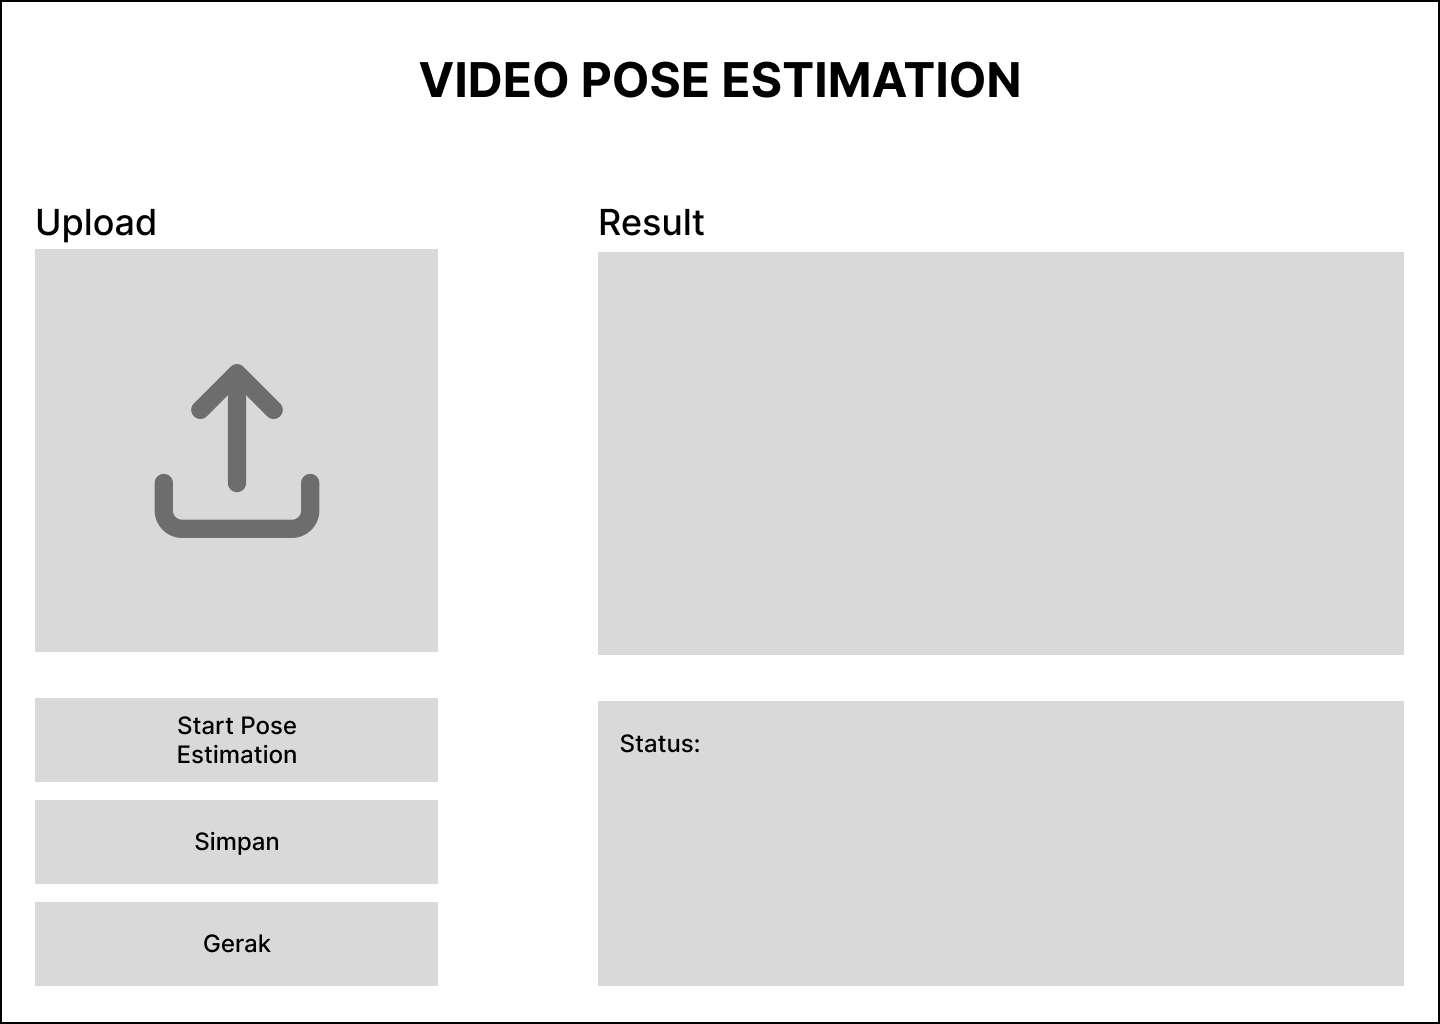
\includegraphics[width=0.8\textwidth]{images/Wireframe - 1.png}
    \caption{Perancangan Antarmuka Sistem}
    \label{fig:wireframe_ui}
\end{figure}

Gambar \ref{fig:wireframe_ui} menunjukkan rancangan awal antarmuka pengguna (UI) dari sistem yang dikembangkan. Antarmuka ini dirancang dengan tampilan yang sederhana dan intuitif untuk mendukung alur kerja mulai dari proses unggah video, estimasi pose 3D, hingga pengendalian gerak robot humanoid.

Di bagian kiri antarmuka terdapat elemen unggah video yang memungkinkan pengguna untuk memilih dan memasukkan video tari tradisional yang akan dianalisis. Setelah video berhasil diunggah, pengguna dapat memulai proses estimasi pose dengan menekan tombol "Start Pose Estimation". Proses ini akan mengaktifkan model \textit{pose estimation} untuk menghasilkan koordinat 3D dari setiap titik sendi tubuh manusia dalam video.

Hasil estimasi kemudian divisualisasikan pada area di sisi kanan antarmuka dalam bentuk tampilan \textit{3D skeleton}. Visualisasi ini memberikan gambaran postur dan gerakan tubuh dari objek dalam video secara menyeluruh berdasarkan estimasi pose yang telah dilakukan.

Setelah proses estimasi selesai, pengguna dapat menyimpan hasilnya dengan tombol "Simpan". Hasil yang disimpan berupa file JSON yang berisi informasi pose 3D dan sudut servo yang telah dihitung. Tombol "Gerak" digunakan untuk mengirimkan data gerak tersebut ke robot ROBOTIS-OP3 melalui sistem komunikasi ROS, sehingga robot dapat menirukan gerakan berdasarkan data yang telah diproses.

Di bagian bawah kanan antarmuka terdapat area status yang menampilkan informasi proses secara langsung, seperti log atau keluaran terminal. Area ini memberikan umpan balik kepada pengguna terkait status estimasi, penyimpanan data, maupun proses pengiriman ke robot, sehingga memudahkan dalam memantau dan mengontrol seluruh jalannya sistem.

\section{Perancangan Modifikasi Hardware}

Robot humanoid ROBOTIS-OP3 yang digunakan dalam penelitian ini merupakan platform robot terbuka yang dilengkapi dengan aktuator servo pada berbagai sendi tubuh. Namun, dalam bentuk standarnya, konfigurasi pergerakan tangan pada OP3 masih terbatas. Secara default, masing-masing lengan robot hanya memiliki tiga \textit{degree of freedom} (DoF), yaitu:
\begin{itemize}
    \item 2 DoF pada bahu (\textit{shoulder pitch} dan \textit{shoulder roll}),
    \item 1 DoF pada siku (\textit{elbow flexion}).
\end{itemize}

Konfigurasi ini cukup untuk gerakan dasar, namun belum mencukupi untuk mengekspresikan variasi gerakan tangan yang kompleks, seperti yang banyak ditemukan pada gerakan tari tradisional Indonesia yang menuntut rotasi pergelangan atau variasi gerak lengan secara lebih bebas.

Oleh karena itu, dilakukan modifikasi terhadap bagian tangan robot dengan menambahkan satu derajat kebebasan tambahan pada sendi siku berupa \textit{elbow twist}. Dengan penambahan ini, lengan robot memiliki total empat derajat kebebasan sebagai berikut:
\begin{itemize}
    \item 2 DoF pada bahu: \textit{pitch} dan \textit{roll},
    \item 2 DoF pada siku: \textit{flexion} dan \textit{twist}.
\end{itemize}

Penambahan DoF pada siku memungkinkan lengan robot untuk melakukan gerakan rotasi aksial, seperti memutar lengan bawah atau menyesuaikan arah tangan, yang sangat penting dalam meniru ekspresi gerak tangan pada tari tradisional. Modifikasi ini dilakukan dengan menambahkan satu motor servo tambahan yang dipasang secara koaksial pada sambungan siku, serta penyesuaian desain fisik dudukan servo agar tetap sesuai dengan struktur mekanik robot.

Modifikasi ini juga disertai dengan penyesuaian pada sistem kontrol dan inverse kinematics agar sistem dapat mengenali dan mengatur sudut baru tersebut. Dengan peningkatan fleksibilitas pada bagian lengan, robot memiliki kemampuan yang lebih tinggi dalam merepresentasikan gestur kompleks secara fisik dan artistik.


